\documentclass[conference]{IEEEtran}
\IEEEoverridecommandlockouts
% The preceding line is only needed to identify funding in the first footnote. If that is unneeded, please comment it out.
\usepackage{cite}
\usepackage{amsmath,amssymb,amsfonts}
\usepackage{algorithmic}
\usepackage{graphicx}
\usepackage{textcomp}
\usepackage{xcolor}
\def\BibTeX{{\rm B\kern-.05em{\sc i\kern-.025em b}\kern-.08em
    T\kern-.1667em\lower.7ex\hbox{E}\kern-.125emX}}

%=================================================================
%====ADDITIONAL PACKAGES & SETTINGS FROM THE ORIGINAL TEMPALTE====
\usepackage{import} % to use \import{../../../content-tex/}{abstract}
\usepackage{todonotes} % USAGE: \todo[inline]{is there a better example from X topic?}
\usepackage{lipsum}  % USAGE \lipsum[2-4]
\graphicspath{{../figures}} %goes to path: figures/
\newcommand{\etal}{\textit{et al. }} % \etal


\begin{document}

\title{
% Diversity, Equity, and Inclusion of Artificial Intelligence and Robotics for children %Fri  7 Jan 23:59:42 GMT 2022
%Piloting Inclusive Workshops of Artificial Intelligence and Robotics for children %Sat  8 Jan 00:12:35 GMT 2022
%Piloting Inclusive Artificial Intelligence and Robotics for Children %Sat 15 Jan 08:44:06 GMT 2022
%Piloting Diversity and Inclusion in Artificial Intelligence and Robotics for Children %Sat 15 Jan 10:33:54 GMT 2022
Piloting Diversity and Inclusion Workshops in Artificial Intelligence and Robotics for Children %Sun 16 Jan 13:14:45 GMT 2022
}

\author{

\IEEEauthorblockN{
    %1\textsuperscript{st} 
    air4children
    }
\IEEEauthorblockA{
    %\textit{dept. name of organization (of Aff.)} \\
    \textit{air4children: Artificial Intelligence and Robotics for Children}\\
    Xicohtzinco, M\'exico \\
    air4children@gmail.com
}

}

% \author{\IEEEauthorblockN{1\textsuperscript{st} Diego Coyotzi-Molina}
% \IEEEauthorblockA{\textit{dept. name of organization (of Aff.)} \\
% \textit{name of organization (of Aff.)}\\
% City, Country \\
% email address or ORCID}
% \and
% \IEEEauthorblockN{2\textsuperscript{nd} Rocio Montenegro}
% \IEEEauthorblockA{\textit{dept. name of organization (of Aff.)} \\
% \textit{name of organization (of Aff.)}\\
% City, Country \\
% email address or ORCID}
% \and
% \IEEEauthorblockN{3\textsuperscript{rd} Donato Perez-Badillo}
% \IEEEauthorblockA{\textit{dept. name of organization (of Aff.)} \\
% \textit{name of organization (of Aff.)}\\
% City, Country \\
% email address or ORCID}
% \and
% \IEEEauthorblockN{4\textsuperscript{th} Dago Cruz}
% \IEEEauthorblockA{\textit{dept. name of organization (of Aff.)} \\
% \textit{name of organization (of Aff.)}\\
% City, Country \\
% email address or ORCID}
% \and
% \IEEEauthorblockN{5\textsuperscript{th} Antonio Perez-Badillo}
% \IEEEauthorblockA{\textit{dept. name of organization (of Aff.)} \\
% \textit{name of organization (of Aff.)}\\
% City, Country \\
% email address or ORCID}
% \and
% \IEEEauthorblockN{6\textsuperscript{th} Leticia Vazquez}
% \IEEEauthorblockA{\textit{dept. name of organization (of Aff.)} \\
% \textit{name of organization (of Aff.)}\\
% City, Country \\
% email address or ORCID}
% }

\maketitle

\begin{abstract}
In this paper, we present preliminary work of a pilot workshop to promote diversity and inclusion in AI and Robotics to children of an range age between 6 to 12 year old.
We pose the challenge of teaching AI and Robotics in low-income countries where scarcity of funding and specialised professional are able to teach such subjects.
In that way, we presented tools based on free and open-source software, open-source hardware and software, open educational resources as well as alternative education programs to promote diversity and inclusion of new technologies. 
We present the design and the pilot of four lessons of the workshop including: (a) to introduce, (b) to teach fundamentals, (c) to link sensor and human body with robots and (d) to wrap up with a showcase presentation.
We finale the paper with conclusions and the challenges for future work.  
\end{abstract}

\begin{IEEEkeywords}
    Open Educational Resources, Educational robots
\end{IEEEkeywords}

%%%%%%%%%%%%%%%%%%%%%%%%%%%%%%%%%%%%%%%%%
%%%%%%%%%%%%%%%%%%%%%%%%%%%%%%%%%%%%%%%%%
\section{Introduction}
%Guarantee security, accessibly and human dignity are considered the pillars for inclusivity.
Accessible and affordable technology in conjunction with open educational resources can promote equal opportunities for childhood education \cite{yoshie2021-unesco}.
However, teaching state-of-the-art technologies such as Artificial Intelligence and Robotics, AIR, is a current challenge for low-income and often politically or culturally marginalized countries.
Additionally, creating the right environment to promote inclusivity and diversity to teach AIR has been little investigated. 
Astobiza \etal 2019, for instance, reported the need of collaborations between industry and a multidisciplinary group of researchers to address concerns on the paradigm of inclusivity in robotics \cite{MonasterioAstobiza2019}.
In that sense, Astobiza \etal suggested that inclusive robotics should be based on two points: "1) they should be easy to use, and 2) they must contribute to making accessibility easier in distinct environments" \cite{MonasterioAstobiza2019}.
Peixoto \etal in 2018 reported the use of robots as tool to promote diversity leading to improve competences in communication, teamwork, leadership, problem solving, resilience and entrepreneurship \cite{PeixotoCastro2018, PeixotoGonzalez2018}. 
Recently, Pannier \etal in 2020 pointed out the challenges of increasing the  participation of women and underrepresented minorities in the areas of Mechatronics and Robotics Engineering as well as the creation of community of educators to promote diversity and inclusion \cite{Pannier2020}.
Similarly, Pannier \etal mentioned that the prevalence of free and open-source software and hardware made mechatronics and robotics more accessible to a diverse group of population.
Pannier \etal also touched on the importance of offering workshops to different range of underrepresented students leading to inspire other programs and to create outreach activities for students, trainers and workshops \cite{Pannier2020}.
In 2021, we introduced air4children, Artificial Intelligence and Robotics for Children, as a way (a) to address aspects for inclusion accessibility, equity and fairness and (b) to create affordable child-centred materials in AI and Robotics (AIR) in developing countries \cite{montenegro2021air4children}. 
In that sense, another challenge is organising workshops where little is known about the demographics, education and socio-economical variables that impact such communities.
For instance, Xicohtzinco, Tlaxcala M\'exico, is a town of a total population of 14,197 (6762 males and 7435 females) based on The National Institute of Statistics and Geography (INEGI)'s census.
However, the census do not provide number of schools but based on the current habitants, we understand that that there are three public schools including kinder-garden, primary, secondary and high-school; and three private schools including primary and secondary schools. 
% NOT QUITE SURE ABOUT THIS SPECULATIONS:
%What it is not known from the 2020 census is the education levels of the population but our anecdotal experience and from current habitants can tell that the population is a mixture of young professionals and working class population.
That said, we hypothesised that piloting workshops of air4chidren in a town such as Xicohtzinco might led us to have better understanding of the needs and challenges of promoting diversity and inclusion of state-of-the-art technologies with open education resources.

This short paper is organised as follows:
Section II presents Tools to promote Diversity and Inclusion in AI and Robotics for children.
Section III presents the design of workshops for children from 6 to 8 years old.
Section IV presents outcomes of a four lessons pilot workshop for 14 children and the help of three instructors and three supervisors. 
We present results of the workshops and finalise it with conclusions and future work.

%BLURS
% in Artificial Intelligence and Robotics (AIR).
% to encourage children to discover and increase their interest in 
% to promote of air4children and to create the inclusive and diversity environments might led us to have better understanding of the current needs and might provide with further evidence 
% of the real needs of the community. 
%we design and pilot workshops of air4children to test how children of different ages and genders and instructors engage to create an environment of diversity and inclusion. 


%%%%%%%%%%%%%%%%%%%%%%%%%%%%%%%%%%%%%%%%%
%%%%%%%%%%%%%%%%%%%%%%%%%%%%%%%%%%%%%%%%%
\section{Tools to promote Diversity and Inclusion in AI and Robotics for children}
\todo[inline]{MX: this section/subsection requires to be refined by adding perpahs other references and align it to air4children}

\subsection{Free and open-source software, open-source hardware and open educational resources}
Recently, Montenegro \etal presented examples to create educational resources aimed to be "affordable, educational and fun", such examples are Otto DIY -- an educational open source robot and JetBot platform -- open source educational robot to create new AI projects \cite{montenegro2021air4children}.
In that sense, Otto Humanoid is a good option for our work because of its affordability costing of 200 EUROS, a block diagram programming interface, the multiple sensors and actuators (servos and LCD matrix display) aligned with open-source software and hardware principles \cite{OttoDIY:2016}.
Similarly, Open Educational Resources (OER) aiming to provide "teaching and learning materials that are available without access fees" seems to be a right direction to afford innovation through OER-enabled pedagogy \cite{Clinton-Lisell2021}.
Wiley \etal in 2014 stated that one of the benefits of OERs is to make course development process quicker and easier but also highlighting the challenges of making OER material for people easier to find but with the challenge of making financially self-sustainable programs among many other difficulties \cite{Wiley2014}.

\subsection{Alternative education programs with new technologies}
Alternative education programs such as Montessori, Waldorf and Regio Emilia considers children as active authors of their own development \cite{edwards2002}.
These programs have been well adopted internationally; however Edwards \etal pointed out the schools deriving from the same philosophy might also need to observe teacher-child interactions, its environments and interview to the past and present parents and children \cite{edwards2002}.
Similarly, in the last 5 years such programs are starting to include topics on AI, robotics and computational thinking into their curriculum \cite{elkin2014, Aljabreen2020}.
For instance, Aljabreen pointed out the adoptions of new technologies and how early child education is re-conceptualised \cite{Aljabreen2020}. 
Elkin et al. in 2014 explored the how robots can be used in the Montessori curriculum \cite{elkin2014}.
Similarly Elkin et al. posed the question on the revision of new curriculums that include technology should not deviate from the main purpose of the Montessori classroom \cite{elkin2014}.
Drigas and Gkeka in 2016 reviewed the application of information and communication technologies in the Montessori Method, mentioning the Manipulatives, as objects to develop motor skills or understand mathematical abstractions, are based on cultural areas, language, mathematics and sensoria but little to none on technological areas \cite{DrigasGkeka2016}.
Drigas and Gkeka reviewed Montessori materials of the 21st century where interactive systems with sounds and lights, touch application to enhance visual literacy or the development of computational thinking and constructions of the physical world \cite{DrigasGkeka2016}.
These indicate that the incorporation of such manipulatives with the use of robotics might led to reach scenarios to explore motor skill development, visualisation and computational thinking. 
Recently, Scippo and Ardolino reported a longitudinal study of the use of computational thinking in five years participants of primary school in a Montessori school \cite{ScippoArdolino2021}
Scippo and Ardolino pointed out the importance of alignment of the Montessori material with the computational thinking activities. 

That said, previous authors stated various challenges on the incorporation of new technologies into their curriculum posing more questions on creating curriculums that should be more accessible to a diverse group of population as it is done in the case of open educational resources.


%%%%%%%%%%%%%%%%%%%%%%%%%%%%%%%%%%%%%%%%%
%%%%%%%%%%%%%%%%%%%%%%%%%%%%%%%%%%%%%%%%%
\section{Designing Diversity and Inclusion Workshops}
To design diversity and inclusive workshops we were considered the six ideas discussed in "Ensuring education and Inclusive Learning for Educational Recovery 2021" \cite{opertti2021-unesco} and 
‘Concrete to abstract’ concept within the Montessori philosophy \cite{MontessoriBOOK1969}.
In one hand, we considered the six ideas to ensuring and inclusive learning summarised as:
(1) personalisation of education including the recognition of specific learning expectations and needs,
(2) designing inclusive, emphatic and participatory curriculum for an plural and open participation of a diversity of actors and institutions,  
(3) appropriation of technology as a community resource to strength ties between students, educators, families and communities,  
(4) empowering knowledge, learning, collaboration, trust and listening among peers, and
(5) the visualisation of schools as lifelong learning spaces.
On other hand, the workshop were planned to develop concepts and skills using 'concrete' concept with hands-on learning materials to make abstract concepts clearer as it is taught in Montessori education \cite{MontessoriBOOK1969}. 

That said, with the combination of Open Educational Resources, alternative education programs and the six ideas, we designed a four lesson workshop with two-fold aims:
(a) to promote diversity of and inclusion to children to teach AI and Robotics and 
(b) to encourage children to discover and increase their interest in AI and Robotics. Figure \ref{fig:curriculum} presents four lessons of the workshops.

\begin{figure}[t]
    % \centerline{\includegraphics[width=\linewidth]{figures/curriculum.png}}  %%OVERLEAF
    \centerline{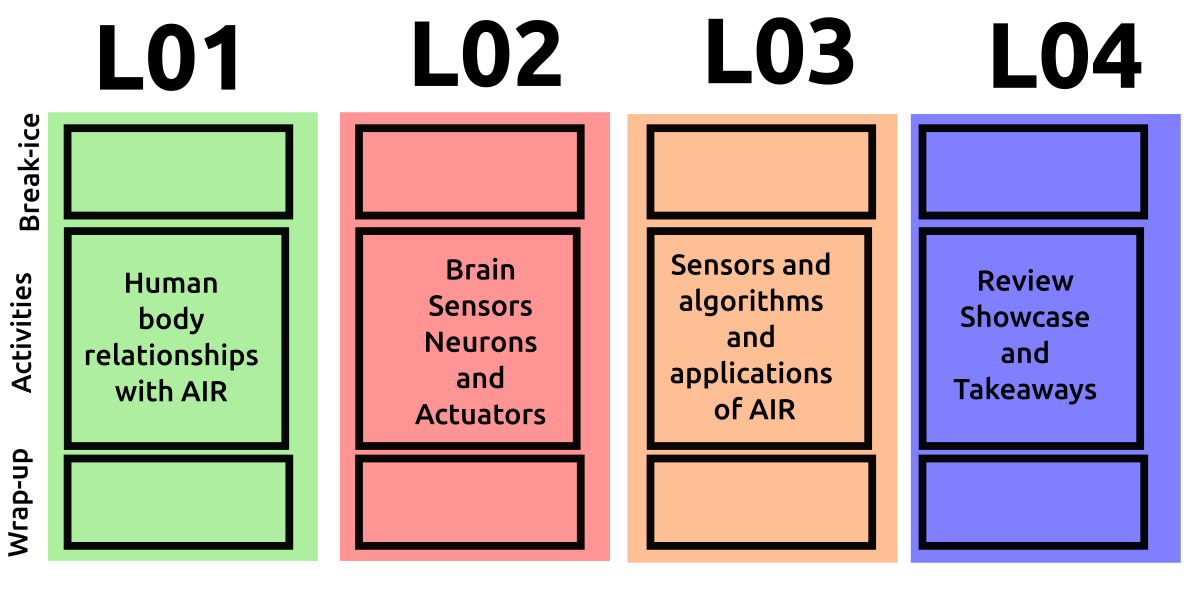
\includegraphics[width=\linewidth]{curriculum-design/versions/drawing-v01.png}}  %%GITHUB
    \caption{Curriculum for four lessons (L01 to L04). 
    Lesson 01 introduce the course, 
    lesson 02 provides the basics of anatomy, 
    lesson 03 covers algorithms, and 
    lesson 04 wrap-up and showcase the project of children.
    }
    \label{fig:curriculum}
\end{figure}

\paragraph{Lesson 01: Breaking the ice and motivations} 
The educational goal for this lesson was to develop the children’s curiosity about AI and Robotics while emphasizing the importance of interpersonal connections that will evolve into a collaboration work for the following lessons.
That said, this lesson started with a recreational activity where each student and teacher introduced themselves with name, favorite food and a superpower or ability that we would like to have and that was related to robots. This lesson also covers basic concepts and examples of AI and Robotics in different fields and daily life, how the brain works and how the human senses and body parts relates to the way a robot is built and how it works and perform activities.

\paragraph{Lesson 02: Human senses and coding my first robot} 
The main purpose of this lesson was to understand fundamentals of Robotics. 
Children began to work with more abstract concepts, developing problem-solving skills as well as cooperatively working relationships. 
The first activity, outside of the classroom, was a true or false game, were the teacher told a sentence about AI and Robotics, and the children jumped in front of a rope if the sentence was true, or if the sentence was false, the kids jumped behind of the rope.
In the second activity, the instructor explain about the human senses and their relationship with inputs and outputs. After that, instructors explain examples of sequences and codes. 
In the last activity, participants were asked to sort out tangram in a group in which a leader of the group provide instructions to the team-mates as an analogy of coding a robot with algorithms.

\paragraph{Lesson 03: Playing with reaction-action activities} 
The educational goal of this lesson is to cover the concept of the effect of causes and consequences with daily life examples and the computational thinking of robots.
Hence, this lesson start with a match game consisting of figures and shadow’s figures where participants develop their comparing skills to match similar or different robots.
This lesson covered points on how robot works with sensors, processors, actuators and programming. 
The “find the effect” activity was also introduced where participants have to relate pictures of cause and consequences, for example “the cause is the rain and the consequently is a rainbow”.
Afterwards, we worked with the Otto humanoids in which we programmed the sensor presence for that robot moves, dances and that emit texts with the 8x8 matrix.

\paragraph{Lesson 04: Develop your own AIR}
The four lesson aimed to summaries what was covered in the previous lessons emphasising the relationship of the human body anatomy (brain, neurons and body parts) with humanoid robots (computer, sensors and actuators).
This lesson covered real-word application of AI and Robotics including medicine, spacial robotics and smart cities. 
Three projects were prepared to be introduced to each team in which every participant have a role. 
Each team prepare a short speech of their application using AI and Robotics. 
%%%%%%%%%%%%%%%%%%%%%%%%%%%%%%%%%%%%%%%%%
%%%%%%%%%%%%%%%%%%%%%%%%%%%%%%%%%%%%%%%%%
\section{Piloting Diversity and Inclusion Workshops}
To pilot the four-lesson workshop, we invited 14 participants (6 female and 8 male) with range of age from 6 to 11 years old (average age of 7.64) (Figure \ref{fig:pilot}). 
Three instructors with three years of experience in teaching and two coordinators with ten years of teaching experience volunteered to deliver four lessons of 90 minutes in the workshop (as shown in the proposed curriculum Fig \ref{fig:curriculum}).
During the initial three lessons, children incorporated the gained knowledge to relate fundamental human body anatomy (brain, neurons, body and senses) to robot parts (microcontroller, motors, sensors). In the final lesson, children showcased their final work promoting a sense of achievement in the children working not only with their mind but also with their social emotional well-being. 

\begin{figure}[tbp]
    % \centerline{\includegraphics[width=\linewidth]{figures/workshop.png}} %%OVERLEAF
    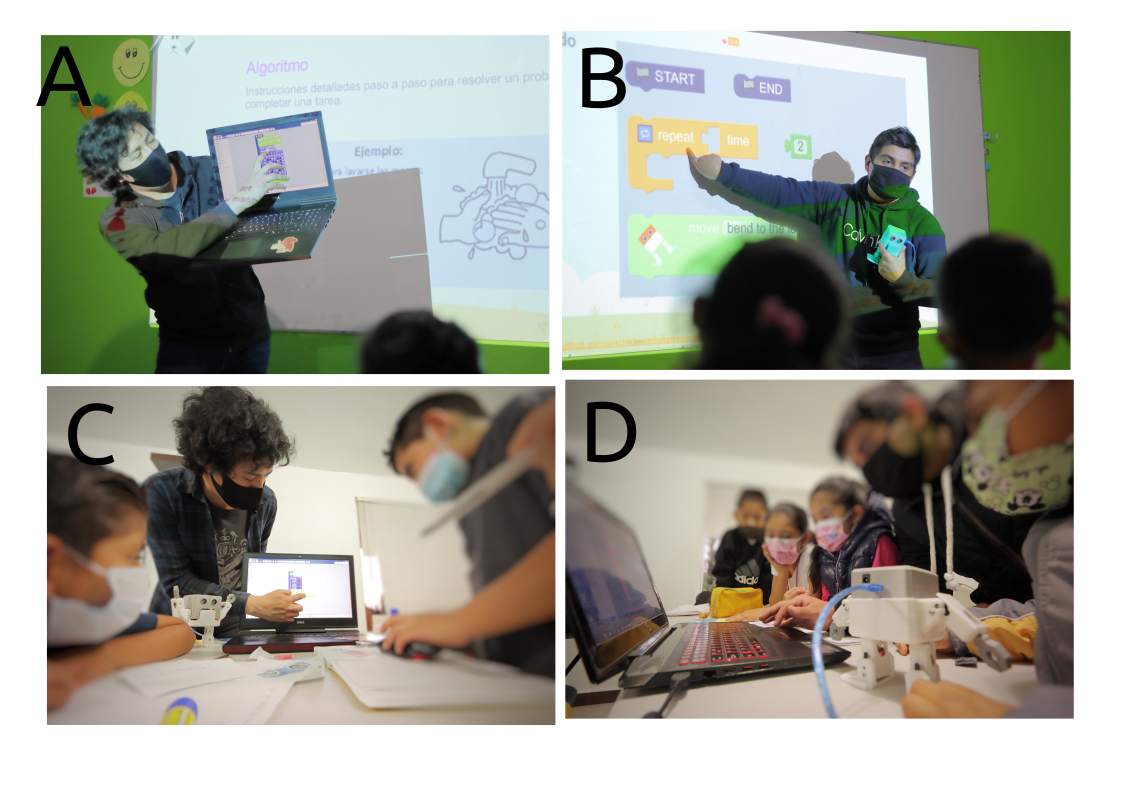
\includegraphics[width=\linewidth]{piloting-workshops/versions/drawing-v00.png} %%GITHUB
    \caption{
        Instructors demonstrating basics of AI and Robotics (A, and B). 
        Children engaging with robots, classmates and instructors (B, and C).
        }
    \label{fig:pilot}
\end{figure}

We however noticed that each lessons was originally planned to be 90 minutes and we did not consider breaks neither perhaps the participant's energy levels to which in the second to four lesson a 15 minutes break was incorporated.
Additionally, we pilot surveys to (a) children with ten questions about their understanding and feelings towards different type of robots and (b) to parents with 30 questions about their understanding of AI and robotics and how parents were aware of  technological advances in AI and Robotics.
Although the aim of the surveys was not to be reported but only to understand how participants and parents feel about being surveyed and how the logistics of surveys would be followed with more participants.
That said, we noticed that participants require support as few participants were not familiar with reading surveys and the content of 10 questions was spread into five questions into two sessions.
On other hand, parents thought that surveys were lengthy taking more than 60 minutes and we also realised that a paper-based survey require more work as scans and transcripts are required. 


% \begin{table}[htbp]
%     \caption{Table Type Styles}
%     \begin{center}
%     \begin{tabular}{|c|c|c|c|}
%     \hline
%     \textbf{Table}&\multicolumn{3}{|c|}{\textbf{Table Column Head}} \\
%     \cline{2-4} 
%     \textbf{Head} & \textbf{\textit{Table column subhead}}& \textbf{\textit{Subhead}}& \textbf{\textit{Subhead}} \\
%     \hline
%     copy& More table copy$^{\mathrm{a}}$& &  \\
%     \hline
%     \multicolumn{4}{l}{$^{\mathrm{a}}$Sample of a Table footnote.}
%     \end{tabular}
%     \label{tab1}
%     \end{center}
% \end{table}
    


%%%%%%%%%%%%%%%%%%%%%%%%%%%%%%%%%%%%%%%%%
%%%%%%%%%%%%%%%%%%%%%%%%%%%%%%%%%%%%%%%%%
\section{Conclusions and future work}
In this paper, we investigate the challenges of Diversity and Inclusion to teach "Artificial Intelligence and Robotics for Children" with open educational resources and principles of Montessori education. 
For the design and the pilot of the workshop, we invited 14 children of an average age of 7.64 years old participated of the community of Xicohtzinco Tlaxcala Mexico.
The workshops were free of cost as a way encourage participation of anyone. 
During the pilot workshop, children were enthusiastic about learning the fundamentals for AIR by building, coding, designing and playing with open-sourced robots. The instructors embraced the different set of skills each child had by working in small groups and supporting the students during the process. These lessons intended to remain beyond the learning of a single concept and contribute to develop a skill the children can take and apply to other areas in their life.
However, we noted that grouping children of four participants with one instructor was not creating an engaging experience as each group has only one robot and one computer and the space and number of participants was leaving sometimes one participant outside of the reachable robot-computer setup.
As a future work, we are planing to organise another workshop in the four quart of the 2022 where we will consider 10 lessons distributed in four weeks with we will invite more participants.
For curriculum of the workshops, we will improve the interactivity of the participants and create more engaging and inclusive activities. We will incorporate a similar approach of the synthesis program which aim is to cultivate student voice, strategic thinking and collaborative problem solving \cite{synthesis2022}.
%started in 2014 with Josh Dahn and support of Elon Musk, 



\section*{Acknowledgment}
To Rocio Montenegro for her contributions with the design of the Montessori curriculum for the workshops.
To Marta P\'erez and Donato Badillo for their support in organising the pilot of the workshops.
To Donato Badillo-Per\'ez, Antonio Badillo-Per\'ez and Diego Coyotzi-Molina for volunteering as instructors of the workshops.
To Leticia V\'azquez for her support with the logistics and feedback to improve the workshops.
To Adriana P\'erez-Fortis for her contributions and discussion to prepare draft surveys for the parents and children. 
To El\'ias M\'endez Zapata for his support and feedback on the hardware design of the robot.
To Dago Cruz for his feedback and discussions on the design of the workshops.
To Angel Mandujano, Elva Corona and others who have contributed with feedback and support to keep iterating the project of AIR4children. 


\section*{Contributions}
Antonio Perez-Badillo: Contributing to design and write up of lesson 02.
Dago Cruz:
Diego Coyotzi-Molina: Contributing to design and write up of lesson 03.
Donato Perez-Badillo: Contributing to design and write up of lesson 01.
Leticia Vazquez: Write up and refinement of the conclusions.
Miguel Xochicale: Contributing to create the template, drafting, write-up, edition, and submission of the paper. 
Rocio Montenegro: Contributing to the write up of designing and piloting workshops. 

\bibliographystyle{IEEEtran}
% \bibliography{references} %%OVERLEAF
\bibliography{../references/references} %%GITHUB


\end{document}
